\chapter{更多电路专题}

在前面我们已经学习了所有电路原理。在这一章中我们以电路功能分类,介绍一些常用的电路模块。当然在这之前,我们需要详细地了解泰拉瑞亚中所有电路物品的性质,这样才能知道我们可以做什么。泰拉瑞亚wiki中当然包含每个电路物品的词条,所以这里仅对wiki中没有的信息进行补充。

\section{电路物品介绍}\label{dianluwupinjieshao}

\subsection{电线、分线盒}
电线没什么好讲的,这里为了方便看电路,提供电线的15种颜色(包括不同色电线重叠显示的颜色)作参考(\autoref{i203})。

\begin{figure}[!h]
\centering

\includegraphics{images/203.png}
\caption{四列分别是:无红线无蓝线、有红线无蓝线、无红线有蓝线、有红线有蓝线。四行分别是:无绿线无黄线、有绿线无黄线、无绿线有黄线、有绿线有黄线。}
\label{i203}
\end{figure}

分线盒可任意摆放,不需要支撑块和背景墙。分线盒可以使交叉的同色电线不接通。锤击分线盒可以改变分线方式,分线方式从分线盒外观可以直观看出。

\subsection{开关/控制杆}
开关和控制杆的激活条件是鼠标右击。同其他交互类物品/NPC相同,只有当开关/控制杆在可触及范围内时才可以右击。

与控制杆相比,由于开关体积更小,在电路密集时一般都使用开关。另一方面,小的体积带来的缺点是开关不容易发现,而且容易点错。

开关可以放置在木梁侧面与前景物块侧面而控制杆不行;控制杆可以放置在平坦表面上而开关不行(\autoref{i204})。需要注意的是,只有当砧上有足够面积的背景墙时,控制杆才可以放置在砧上,放置在砧上后敲掉背景墙也不会掉落,这可能是判定的bug。

\begin{figure}[!h]
\centering

\includegraphics[width=0.9\textwidth]{images/204.png}
\caption{放置在平坦表面上的控制杆}
\label{i204}
\end{figure}


\subsection{压力板}
压力板分为普通压力板、加重压力板、青绿压力垫板。

普通压力板包括由玩家触发的灰/棕/蓝/丛林蜥蜴压力板、由敌怪触发的黄压力板和由玩家或敌怪触发的红/绿压力板。加重压力板是误翻译,正确翻译应为“重力压力板”。四种颜色的加重压力板功能完全一样。

普通压力板有自身的碰撞箱,碰撞箱大小是压力板弹起状态时贴图的边框大小。普通压力板激活的判定以每个碰撞箱为准,即每帧判定碰撞箱是否从侧面进入压力板,或从上面掉落到压力板上。因为是以碰撞箱为准,所以一个碰撞箱在一帧内触发两个普通压力板,只会激活一次,而不同碰撞箱在一帧内触发同一个普通压力板,每个碰撞箱都会激活一次(\autoref{i205:208})。注意到“进入”或“掉落”都是过程,所以直接传送到普通压力板上不会触发压力板。同时,“掉落”要求人物有一个悬空的过程,判断悬空可以通过人物动作(悬空时有跳跃动作)或者翅膀(装备了翅膀的人物悬空时翅膀会打开)。所以从1格高的物块上直接走下来不算掉落,同时碰撞箱也不是从侧面进入,所以不会触发普通压力板(\autoref{i201:202})。

\begin{figure}[!h]
\begin{center}
\subfloat[]{
\label{i205:206}

\includegraphics{images/205.png}

\includegraphics{images/206.png}
}
\qquad
\subfloat[]{
\label{i207:208}

\includegraphics{images/207.png}

\includegraphics{images/208.png}
}
\end{center}
\caption{\protect\subref{i205:206}同时踩踏两个红压力板,只有左边的火把响应;\protect\subref{i207:208}虚化两个NPC脚下的方块,两个NPC同时掉落到红压力板上,火把仍亮。}
\label{i205:208}
\end{figure}

\begin{figure}[!h]
\begin{center}
\subfloat[]{
\label{i201}

\includegraphics{images/201.png}
}
\qquad
\subfloat[]{
\label{i202}

\includegraphics{images/202.png}
}
\end{center}
\caption{\protect\subref{i201}直接从一格高度走下,翅膀不打开,无跳跃动作,压力板不会被触发;\protect\subref{i202}在平台上按“下”方向键,翅膀打开,有跳跃动作,压力板会被触发。}
\label{i201:202}
\end{figure}

加重压力板没有碰撞箱,判定以压力板本身为准,即每帧或者每次传送后判定是否有人物在压力板所在格内,直接传送到加重压力板上可以触发加重压力板。为避免冲突,加重压力板的激活信号及以该信号触发的逻辑结算产生的激活信号不会触发传送机。

青绿压力垫板的碰撞箱为16*10或10*16,根据其朝向而定。射弹生成后,每次更新位置都会激活碰撞到的青绿压力垫板,这里碰撞的定义是:上次更新时碰撞箱不相交,但是这次更新时相交。如果射弹同时与多个青绿压力垫板碰撞,那么只激活优先级最高的那个(不同行的青绿压力垫板,上面的优先级高;同一行的青绿压力垫板,左边的优先级高);多个射弹同时碰撞同一个青绿压力垫板,每个射弹都会激活一次(\autoref{i209:212})。

\begin{figure}[!h]
\begin{center}
\subfloat[]{
\label{i209:210}

\includegraphics{images/209.png}

\includegraphics{images/210.png}
}
\qquad
\subfloat[]{
\label{i211:212}

\includegraphics{images/211.png}

\includegraphics{images/212.png}
}
\end{center}
\caption{\protect\subref{i209:210}大炮发射,只有左边的火把响应;\protect\subref{i211:212}激活左边或右边的开关火把都响应,激活中间的开关火把不响应(实际上响应了两次)。}
\label{i209:212}
\end{figure}

普通压力板和加重压力板可以放在平台和锭上而青绿压力垫板不能;青绿压力垫板可以放在前景物块侧面和下方而普通压力板和加重压力板不能。

压力板轨道是带有压力板的轨道,它只能由矿车触发。

\subsection{引爆器}
引爆器是一个比较特殊的物品,其有压下和弹起两种状态。鼠标右击或人物以至少3像素/帧的垂直速度经过引爆器上两格时会导致引爆器压下并作为电源激活,随后经过1秒,引爆器自动弹起。可能出于判定原因,当人物以一定速度(既不快也不慢)落在引爆器旁边的支撑物边缘时引爆器也会压下(\autoref{i213:214})。引爆器处于压下状态时鼠标右击或人物踩踏均无效(贤者模式)。

\begin{figure}[!h]
\begin{center}
\subfloat[]{
\label{i213}

\includegraphics{images/213.png}
}
\qquad
\subfloat[]{
\label{i214}

\includegraphics{images/214.png}
}
\end{center}
\caption{\protect\subref{i213}站在平台边缘原地跳跃,当跳跃高度在某个范围内时,落下会踩下引爆器;\protect\subref{i214}骑乘坐骑也有这种现象。}
\label{i213:214}
\end{figure}


引爆器同样也是用电器,被激活时会在压下和弹起之间切换。如果引爆器被激活压下,那么不会作为电源激活,也不会自动弹起,直到再次被激活弹起。

引爆器可以放在几乎所有平坦表面上。与控制杆不同的是,引爆器不是悬挂家具,所以不能放在砧上。

\subsection{受困宝箱}
受困宝箱是误翻译,正确翻译应该是“机关宝箱”或“陷阱宝箱”。受困宝箱是电源,当鼠标右击时激活并播放宝箱开启关闭的动画。除了右击效果不同以外,受困宝箱与对应的普通宝箱外观、放置方式完全相同,这使得受困宝箱可以用来做陷阱的触发器。

\subsection{感应器}
泰拉瑞亚中共有3种逻辑感应器和4种液体感应器。逻辑感应器(昼)在白天点亮,夜晚熄灭;逻辑感应器(夜)在白天熄灭,夜晚点亮;逻辑感应器(玩家)放置时对应一个电路层的蓝色方框,该方框宽略大于5格,高略大于10格,当框内有玩家时感应器点亮,当框内无玩家时感应器熄灭。液体感应器在所在格中有对应液体时点亮,无对应液体时熄灭。

逻辑感应器(昼)和逻辑感应器(夜)在由灭变亮时激活,其他感应器均在亮灭切换时激活。

逻辑感应器(玩家)可以看作感应范围更大,但是对传送不敏感,仅在每帧进行判断的加重压力板。逻辑感应器(玩家)的激活信号及以该信号触发的逻辑结算产生的激活信号不会触发传送机。

所有感应器均可随意放置,无需支撑块或背景墙。

使用地图编辑器或Mod复制粘贴的感应器无法工作,需拆除后手动放置。因此设计电路时应尽量避免大规模使用感应器。

\subsection{逻辑门、逻辑灯}
逻辑门可随意放置,无需支撑块或背景墙。

逻辑灯只能放置在逻辑门上或其他逻辑灯上。破坏逻辑门会使得其上所有逻辑灯破坏;破坏逻辑灯也会使其上的所有逻辑灯破坏。

\subsection{部分光源}
这里说的光源不是指有效光源,而是指所有能发光的物体。所有可由电路控制的光源如下列举。

\begin{itemize}
\item 火把:大小1*1,放置在平台上、前景物块上方和两侧、背景墙上。是有效光源。
\item 蜡烛:大小1*1,放置在除砧以外的平坦表面上,可以放置在锭上但会立刻掉落。水蜡烛和和平蜡烛无电路功能。是有效光源。
\item 灯笼:大小1*2,悬挂在前景物块下。萤火虫瓶和荧光虫瓶无电路功能。星星瓶和红心灯笼熄灭时不提供buff。是有效光源。
\item 灯:大小1*3,放置在平台上、锭上、前景物块上。是有效光源。
\item 篝火:大小3*2,放置在平台上、锭上、前景物块上。熄灭时不提供buff。是有效光源。
\item 烛台:大小2*2,放置在除砧以外的平坦表面上、前景物块上。是有效光源。
\item 吊灯:大小3*3,悬挂在前景物块下。是有效光源。
\item 晶莹宝石块:属于前景物块。不是有效光源。
\item 中式灯笼:大小2*2,悬挂在前景物块下。是有效光源。
\item 灯柱:大小1*6,放置在平台上、锭上、前景物块上。不是有效光源。
\item 迪斯科灯:大小2*2,悬挂在前景物块下。不是有效光源。
\item 圣诞灯:大小1*1,放置在前景物块四周。是有效光源。
\item 壁炉:大小3*2,放置在平台上、锭上、前景物块上。是有效光源。
\end{itemize}

这里需要强调一下常用的两种显示光源:宝石块和火把。一般情况下宝石块显示效果更好,并且其亮灭会显示在小地图中。然而由于火把激活时只是简单改变状态,而每个宝石块激活时还需要更新该块及周围8块的贴图,每次更新贴图时都需要进行大量的判断,这导致大规模使用宝石块的电路与使用火把的电路相比非常卡。

\subsection{门、机关门、高门}
上锁的丛林蜥蜴门无电路功能(废话)。门放置在上下两个前景物块之间。图格、生物出现在门一侧的开启范围内(1*3)时门不会向这一侧开启;出现在门两侧开启范围内时门无法开启。当门可以向两侧开启时,如果右键开门,那么门向玩家面对方向开启;如果电路开门,那么门似乎是随机向两侧开启。

与门相比,机关门的开启方向是上下。当机关门可以向两侧开启时,使用右键开门,根据玩家与门的相对位置确定开门方向:玩家在相对高处时门向下开启;玩家在相对低处时门向上开启。使用电路开门,固定向下开启。

高门没有方向性,开门也不受阻挡。

\subsection{泵}
用一根电线连接一个入水泵和一个出水泵,则电线激活时,入水泵上的液体会尽可能多的转移到出水泵。

为了了解一些奇怪情况下的液体转移结算,这里介绍水泵的内部运行机制。

游戏中用两个长度19的列表分别存储入水泵和出水泵的坐标。在这个列表中,每个泵都是单个图格。游戏中的泵包含四个图格,当该泵被激活时,四个图格被依次加入列表中,顺序是左下-右下-左上-右上。加到列表满时则不继续加入。

每根电线结算完成后进行水泵结算,从前往后扫描入水泵列表(没有液体的入水泵除外),对于每个入水泵,从前往后扫描出水泵列表(满液体的出水泵除外),并对入水泵和出水泵中的液体进行转移。

单格入水泵和单格出水泵之间的液体转移,首先要遵循液体一致的原则,即转移液体不会导致不同液体出现在出水泵上。其次,转移的量为入水泵上的液体总量和出水泵上空余液体量的最小值(每格中的液体量为0到255)。

\subsection{机关}
这里说的机关指激活会对玩家造成伤害的用电器。

超级飞镖机关、尖球机关、烈焰机关、长矛机关都生成在丛林蜥蜴神庙内。飞镖机关生成在地下其他位置。这5种机关属于前景物块,锤击可以改变射击方向;被激活会生成射弹,可触发青绿压力垫板。

飞镖机关、超级飞镖机关、尖球机关和烈焰机关的射弹在机关前方第2格生成,因此紧贴这4种机关前方的一个前景物块不会阻挡射弹。紧贴长矛机关前方的前景物块会阻挡长矛。

飞镖在真空中的速度是每秒45格,生存时间60秒。飞镖机关、超级飞镖机关和烈焰机关的冷却时间是200帧。

长矛机关射程19.5格\footnote{由@dcfhft 验证。},冷却时间90帧。

烈焰机关射程20格,冷却时间200帧。尽管烈焰机关的特效较宽,其射弹仍只在机关正前方生成。

尖球机关冷却时间300帧,有生成限制。其限制规则较复杂,请参阅wiki。

因为翻译原因,喷泉(机关)在中文wiki中无法查到,因为与喷泉(装饰)冲突\footnote{喷泉(Geyser)是自然景观,喷泉(Fountain)是人造景观,官中并未区分翻译。}。请在英文wiki中查阅Geyser词条。

喷泉(机关)可放置在前景物块上或下,其朝向也根据放置位置分为朝上和朝下。冷却时间200帧。不会触发青绿压力垫板。射程20格,射程从喷射方向29格内遇到的第一个2*4开放空间(没有前景物块和液体)开始,其后会被障碍物阻挡。

炸药被激活时爆炸,爆炸半径10格。炸药是一次性的,所以在电路中应用有限。使用地图编辑器或Mod可以将炸药放在宝箱下,由于宝箱下的物块无敌,炸药可以被无限引爆。

地雷被激活时爆炸。与炸药的区别是地雷不破坏图格,伤害也更低。另一方面,地雷被玩家或NPC踩踏时也会爆炸,这使得引爆地雷可以不用电线,因此可以通过刷漆使地雷完全不可见。

\subsection{炮台}
炮台包括大炮、兔兔炮、彩纸炮、传送枪站和雪球发射器。

炮台大小为4*3,但是可以放置在两格宽的前景物块、平台或锭上。

鼠标右击炮台左/右部分可转向,拿着对应炮弹左击可发射。使用电线激活时,激活炮台的不同位置有不同效果(\autoref{i215})。使用电线激活发射的炮弹不造成伤害。

炮台生成射弹的位置横坐标在中间两列的交界,纵坐标在下面一格与中间一格的交界。对于传送枪台,生成位置还要向下移5像素;如果传送枪台朝向垂直向上,生成位置还要向右移5像素。

炮台生成射弹的初速度大小,传送枪站为93像素/帧\footnote{具体为每次前进3像素,每帧前进31次},其他为14像素/帧。初速度方向只与炮台朝向有关,除了0、$\pi/2$、$\pi/4$的特殊角以外,非特殊角分别为$\arctan(1/3)$和$\pi/2-\arctan(1/3)$而不是$\pi/8$和$3\pi/8$。

大炮和兔兔炮的炮弹射出后,前17帧速度不变,从第18帧开始,每帧纵向速度增加0.28像素/帧(最大16像素/帧),横向速度乘0.99。传送枪台的射弹匀速直线运动,并会按顺序激活路径上的所有青绿压力垫板。彩纸炮发射的射弹匀速直线运行,生存期为2帧,生存期结束后爆炸,生成特效。在这2帧内,射弹只能前进28像素,无法离开炮台4*3的大小,也就无法触发青绿压力垫板。

\begin{figure}[!h]
\centering

\includegraphics{images/215.png}
\caption{红线右转,蓝线左转,绿线发射,黄线改变射弹颜色。}
\label{i215}
\end{figure}

传送枪站的鼠标操作与其他炮台不同。鼠标右击传送枪站不同位置效果与电线激活对应位置相同。

除彩纸炮以外的炮台发射的射弹可以触发青绿压力垫板。冷却时间30帧。

雪球发射器较特殊,其特性与以上描述几乎完全不同。雪球发射器大小3*3,只能放置在三格宽的前景物块、平台或锭上。雪球发射器不可手动转向,背包中有雪球时右击可发射雪球,可连发。发射出的雪球可触发青绿压力垫板。使用电路激活其左三格之一会使其朝向左,激活其右三格之一会使其朝向右,激活中间三格之一会发射不造成伤害的雪球。雪球发射器朝向只有两种:水平向左和水平向右。发射点在雪球发射器中心向左12像素(如果朝向左)或向右12像素(如果朝向右);发射速度在[12:0.01:16.49]中随机;发射方向随机(见\autoref{e1})。雪球发出后,前19帧速度不变,从第20帧开始,每帧纵向速度增加0.3(最大16),横向速度乘0.98。冷却时间10帧。

\begin{figure}[h]
\centering
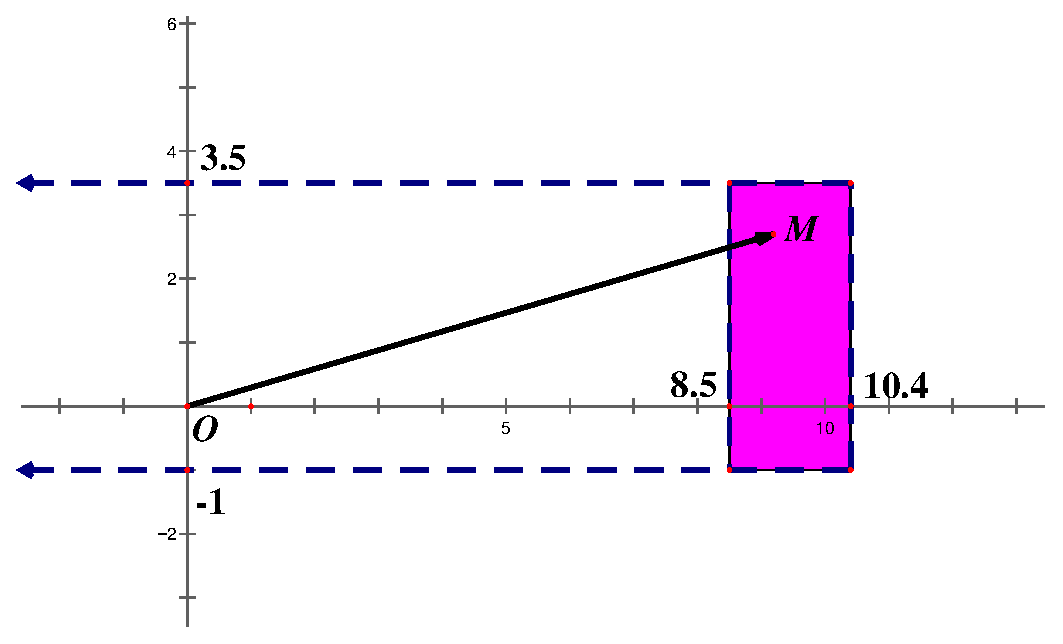
\includegraphics[width=0.9\textwidth]{images/1.eps}
\caption{雪球发射器的发射方向。O为发射点,在如图所示矩形内随机取一点M,则OM为发射方向。}\label{e1}
\end{figure}

\subsection{烟花火箭}
烟花神教主角。关于烟花火箭的信息请参考wiki和\url{https://www.bilibili.com/video/av5050255}。

\subsection{传送机}\label{chuansongji}
一个传送机分为三个图格。传送机为前景物块,可以敲成半砖。传送机的工作机制中,三个图格分别有自己的传送区域(\autoref{i216})。

\begin{figure}[!h]
\centering

\includegraphics{images/216.png}
\caption{三个图格的传送区域。如果图格被敲成下半砖,则传送区域下移半格,其他半砖形态传送区域不变。}
\label{i216}
\end{figure}

当一根电线激活时,记录下该电线下第一个结算的传送机图格与最后一个结算的传送机图格\footnote{同一根电线上的结算顺序请参阅\autoref{jiesuanshunxu}},然后将两个图格传送区域内的可传送目标互换,互换后它们的速度不变,位置相对于传送区域不变。当两个图格的传送区域有重合并且第一个图格不低于最后一个图格时无法传送\footnote{这解释了为什么传送机不会自身传送。};当两个图格的传送区域有重合并且第一个图格低于最后一个图格时可以传送,此时两传送区域重叠部分属于第一个图格的传送区域(\autoref{i217:218})。

\begin{figure}[!h]
\begin{center}
\subfloat{
\label{i217}

\includegraphics[width=0.9\textwidth]{images/217.png}
}
\qquad
\subfloat{
\label{i218}
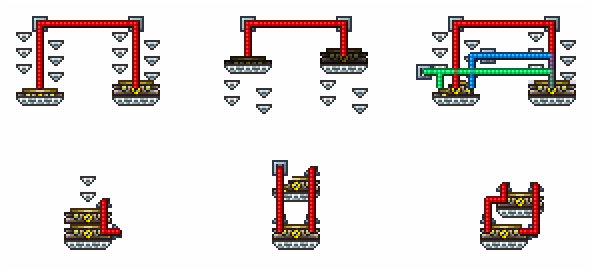
\includegraphics[width=0.9\textwidth]{images/218.png}
}
\end{center}
\caption{左上装置:右边传送机比左边传送机传送区域高半格,因此玩家从左边传送到右边会高半格。中上装置:只要碰撞箱与传送区域有一点重叠,就可以传送。右上装置:传送机的三个图格各自有传送区域,从左边传送到右边,激活绿线会高半格,而激活蓝线红线不会。下方三个装置:激活上面开关不会传送,激活下面开关会传送;传送时只要玩家在下方传送机的传送区域内,就会被从下传到上;传送时只有玩家在上方传送机的传送区域内并且不在下方传送机的传送区域内,才会被从上传到下。}
\label{i217:218}
\end{figure}

\subsection{像素盒}
像素盒可随意摆放,无需支撑块或背景墙。像素盒有十字状态的分线盒的分线效果。当一个电源激活时,该电源上的所有电线激活,此时如果像素盒上有横向电线激活且无纵向电线激活,那么像素盒熄灭;如果像素盒上既有横向电线激活又有纵向电线激活,那么像素盒点亮;如果无横向电线激活,那么像素盒不响应。

需要注意的是,像素盒的响应是对电源敏感的,即分别结算每个电源发出的信号,这与传送机对电线敏感不同。同时,与一般的光源在亮灭之间切换不同,像素盒响应总是调整到对应状态。

\subsection{矿车轨道交叉点}
交叉点上必须有两个方向的平滑轨道,那么这两个平滑轨道必定是一个覆盖另一个,此时激活交叉点会使两个平滑轨道的覆盖关系改变。需要注意的是激活交叉点可以产生的变化远远小于使用锤子可以产生的变化。

\subsection{其他}
剩余的电路物品在wiki之外的信息相当少,因此不专门介绍。它们是:扳手、蓝扳手、绿扳手、黄扳手、钢丝钳、五彩扳手、机械晶状体、精密线控仪、分线盒、计时器、宝石锁、雕像、烟花喷泉、烟花盒、泡泡机、呆萌气球机、派对中心、喷泉、八音盒、烟囱、天塔柱、广播盒、制动器、传送带、彩线灯泡、增速轨道。

有些信息wiki上没有,但是已经确认是正确的。它们是:
\begin{enumerate}
\item 烟花盒的射弹可触发青绿压力垫板。
\item 虚化烟花盒下的物块不会使烟花盒掉落,但是烟花盒的这种悬空状态不稳定。
\item 广播盒可悬挂在敲成下半砖的平台下。
\item 激活有制动器的传送带只会将其虚化,不会使其反向。
\item 彩线灯泡一共有16种状态。
\item 彩线灯泡中心灯泡的颜色是四角颜色的混合,也可以看作电线颜色的混合。
\end{enumerate}

此外,有些信息wiki上没有,且目前尚无研究,待补充。它们是:
\begin{enumerate}
\item 计时器的激活顺序。
\item 长矛机关的弹速。
\item 烈焰机关的射弹信息。
\item 喷泉、八音盒的特效覆盖规律。
\item 各炮台的射弹信息(射速、逐帧轨迹)。
\item 烟花火箭是否会触发青绿压力垫板?
\item 增速轨道提供的加速度。
\item 所有未声明放置方式的道具的放置方式。
\end{enumerate}

\section{驱动与延时器}

驱动与延时器功能和原理都类似,只不过驱动是重复输出,延时器只有一次输出,所以放到一起。

\subsection{降频技术}
灵活使用递次电路和降频电路可以将已有的驱动时长增加为任意整数倍(\autoref{i223:228})。

\begin{figure}[!h]
\begin{center}
\subfloat[]{
\label{i223:224}

\includegraphics{images/223.png}

\includegraphics{images/224.png}
}
\qquad
\subfloat[]{
\label{i225:226}

\includegraphics{images/225.png}

\includegraphics{images/226.png}
}
\qquad
\subfloat[]{
\label{i227:228}

\includegraphics{images/227.png}

\includegraphics{images/228.png}
}
\end{center}
\caption{\protect\subref{i223:224}两个降频电路连接,红线每激活4次火把响应一次;\protect\subref{i225:226}两个递次电路连接,红线每激活9次火把响应一次;\protect\subref{i227:228}降频电路与递次电路连接,红线每激活6次火把响应一次。}
\label{i223:228}
\end{figure}

使用上面的方法,当需要获得较大的质数倍(例如23倍)时间时使用递次电路体积过大,此时可以利用故障逻辑门的控制功能灵活地将多个降频的驱动结合(\autoref{i231:232})。

\begin{figure}[!h]
\begin{center}
\subfloat{
\label{i231}

\includegraphics{images/231.png}
}
\qquad
\subfloat{
\label{i232}

\includegraphics{images/232.png}
}
\end{center}
\caption{开关每激活23次火把响应一次。上面的右边两个故障逻辑门用来控制,左边的输出接到计数为20的模块(5-递次电路与两个降频电路连接),右边的输出接到3-递次电路。开关激活时,起初左边输出,右边不输出,左边计数。当左边计数到20时上面的绿线激活,改变控制用的有效逻辑灯,改为右边输出,左边不输出,右边计数。当右边计数到3时激活火把并将控制用的有效逻辑灯改回。}
\label{i231:232}
\end{figure}

\subsection{计时器串联技术}
将不同时间的计时器连接起来可以得到它们时间之和(\autoref{i229:230})。将相同时间的计时器连接在一起如何呢?

\begin{figure}[!h]
\begin{center}
\subfloat{
\label{i229}

\includegraphics{images/229.png}
}
\qquad
\subfloat{
\label{i230}

\includegraphics{images/230.png}
}
\end{center}
\caption{红线激活后8秒火把激活。红线激活时打开5秒计时器;经过5秒,5秒计时器激活,打开3秒计时器;经过3秒,3秒计时器激活,关闭5秒计时器,激活火把,并通过换线器将自己关闭。}
\label{i229:230}
\end{figure}

wiki告诉我们,当相同时间的计时器A与计时器B连接时,如果A激活将B打开,那么一个计时周期过后,B比A先结算,因此B激活将A关闭,A关闭从而不会激活。因此相同时间的计时器连接在一起也可以得到它们的时间之和(\autoref{i233:234})。灵活结合这个技术与降频技术就可以得到占用体积相当小的整数秒计时器。

\begin{figure}[!h]
\begin{center}
\subfloat{
\label{i233}

\includegraphics{images/233.png}
}
\qquad
\subfloat{
\label{i234}

\includegraphics{images/234.png}
}
\end{center}
\caption{左边红线激活后5秒火把激活。红线激活时打开左一1秒计时器;经过1秒,左一1秒计时器激活,打开左二1秒计时器;经过1秒,左二1秒计时器(在左一1秒计时器之前)激活,关闭左一1秒计时器,打开左三1秒计时器;依此类推。右一1秒计时器激活时关闭右二1秒计时器,激活火把,并通过换线器将自己关闭。}
\label{i233:234}
\end{figure}

\subsection{自定义半砖驱动}
使用假人驱动可以得到60Hz的驱动。如果要进行降频,除了使用降频技术以外,还可以修改半砖装置(\autoref{i235:236})。

\begin{figure}[!h]
\begin{center}
\subfloat[]{
\label{i235}

\includegraphics{images/235.png}
}
\qquad
\subfloat[]{
\label{i236}

\includegraphics{images/236.png}
}
\end{center}
\caption{\protect\subref{i235}只使用一个压力板,频率降为30Hz;\protect\subref{i235}加长半砖,频率降为20Hz。}
\label{i235:236}
\end{figure}

%\subsection{分数帧}
%使用前面的技术得到的时间都是帧的整数倍,即频率一定是60的约数。如果想得到频率不是60的约数的驱动,例如40Hz,50Hz,甚至100Hz,应该怎么做呢?

%首先应该了解到,泰拉瑞亚中物理机制一律以帧为单位。所有驱动,如果要有用的话,都一定是产生某些物理效应,例如发射飞镖、开关火把等。既然这些事件都只能在整数帧发生,那么实际上频率不是60的约数的驱动是不均匀的。

%我们以飞镖为例。飞镖在真空中弹速是每秒45格,冷却时间3 1/3秒,那么如\autoref{}所示,在飞镖机关前面放上150个青绿压力垫板,发射飞镖,则当飞镖触发最后一个青绿压力垫板时飞镖机关应当恰好冷却完毕。将最后一个青绿压力垫板连回飞镖机关就做成了一个驱动。将150个青绿压力垫板用另一种颜色的电线连接并输出就得到了一个理论频率为45Hz的驱动,两个相邻青绿压力垫板激活的间隔应该是1 1/3帧。

%我们使用录制软件将这个驱动的运行过程逐帧回放。

\subsection{随意操纵时间}
我们已经可以利用低频驱动得到任意秒的长时间,使用高频驱动得到任意帧的短时间。将这些装置结合起来就可以得到任意长度的时间。\url{https://www.bilibili.com/video/av13658918}中秒杀拜月教邪教徒就是通过计时器+飞镖机关精确控制时间完成的。

\subsection{其他驱动摘要}
由于使用计时器和假人驱动已经可以随意控制时间,其他驱动也就逐步淡出。但是为了保留思路,仍介绍这些驱动,说不定什么时候有奇效。
\begin{itemize}
\item 生物驱动:利用生物行走速度固定构造的驱动。往往利用雕像刷怪。与玩家距离不能太远,否则生物会消失。雕像怪物速度测试\url{https://www.bilibili.com/video/av22739934}。在1.3.0.1版本引入傀儡之前,半砖驱动一般使用骷髅雕像生成的骷髅。
\item 柱形驱动:利用下层叠平台的稳定间隔构造的驱动。链接\url{https://www.bilibili.com/video/av23028215}。
\item 传送带驱动:已介绍。虽然仍为满频驱动,但是需要限制玩家自由。
\item 机关驱动:利用各种可以发射射弹的电路物品与青绿压力垫板构造的驱动。由于射弹速度各不相同,并且还受液体减速影响,控制不如假人驱动简单。但是由于占用空间可以很小,该类驱动仍有一定价值。
\item 传送机驱动:利用传送机传送对象相对于传送区域位置不变的特性。见\autoref{i219:220}

\begin{figure}[!h]
\begin{center}
\subfloat[]{
\label{i219}

\includegraphics{images/219.png}
}
\qquad
\subfloat[]{
\label{i220}

\includegraphics{images/220.png}
}
\end{center}
\caption{\protect\subref{i219}踩踏红压力板时触发传送机,传送后会悬空一格,坠落到压力板上时继续传送,如此循环;\protect\subref{i220}传送后悬空半格。}
\label{i219:220}
\end{figure}

\end{itemize}

\section{传感器}
泰拉瑞亚中已经自带了很多传感器,例如压力板、感应器等。在实际使用中,我们有时需要检测游戏自带传感器检测不了的东西,那么就需要另外设计传感器。

\subsection{开服感应器}
所谓开服感应器,就是在打开地图时激活的电源。只要地图不关闭,该电源就不会再次激活。

最容易想到的就是在重生点放上玩家感应器,并把玩家传送走。但是这样一来,在玩家回程时会再次激活。使用床传送技术\footnote{\url{https://v.youku.com/v_show/id_XMTg0NzYxNDg0OA}}可以避免这一点,但是无法在退出地图时自动重置。

从打开地图开始,玩家第一次接近傀儡时傀儡影子会在傀儡上生成。傀儡是家具而傀儡影子是敌怪,它们分开结算:家具是固定的,而影子可以移动、受伤害、受debuff。虽然影子不会主动移动,但是会被动移动,例如坠落、传送机传送、半砖传送。当影子受伤害时家具播放动画。影子与家具所在格由于各自的原因均不能摆放前景物块\footnote{前景物块不能摆放在家具图格上或生物碰撞箱上。}。

只要傀儡影子在重生点附近,那么傀儡影子在打开地图时就会重新生成在傀儡上。

最简单的开服感应器如\autoref{i221}。傀儡悬空,下面放有压力板。每次打开地图后傀儡影子生成,掉落在压力板上激活压力板。这个开服感应器略有延迟,延迟长度是傀儡影子掉落到压力板上的时间。一般来说这么短的延迟不会有什么问题。

\begin{figure}[!h]
\centering

\includegraphics{images/221.png}
\caption{}
\label{i221}
\end{figure}

如果想要更短的延迟,可以考虑在开图瞬间用传送机将傀儡影子传送走,并做一些处理使传送机再次激活时不会将影子传送回(\autoref{i222})。

\begin{figure}[!h]
\centering

\includegraphics{images/222.png}
\caption{}
\label{i222}
\end{figure}

上面的装置中,传送机激活后1帧,傀儡影子就被半砖推离传送机并触发红压力板,从而不会再传回。但是玩家感应器和加重压力板不会触发传送机,玩家出生在重生点处也不会触发普通压力板。只能用玩家感应器或加重压力板触发机关,然后用青绿压力垫板激活传送机,这样一来在触发机关到青绿压力垫板激活之间又有一个短延迟。

利用液体可以实现无延迟的开服感应器。打开地图的等待界面中有一项是“正在摆放液体”。这一步是将地图中所有不稳定的液体转移到最低处。在\autoref{i11:12}中,刷水机不断地生成水,水进入到左边的细长通道,并被下面的熔岩轨道吸收。当通道足够长并且刷水速度足够快时,通道中始终有水存在。此时退出地图并重新加载地图时,通道中的水被自动放置到最低处的液体感应器上,从而液体感应器激活。其余部分的功能是:将液体感应器上的水排走;打开刷水的1秒计时器。这个装置的触发是没有延迟的,但是会在游戏中一直运行刷水机,可能影响电脑性能。

\subsection{方向感应器}
方向感应器被广泛地使用在电路游戏中,它可以检测到玩家的上下左右移动操作。方向感应器的一种方案如\autoref{i253:254}所示。另一种方案请参考\url{https://www.bilibili.com/video/av23633364/?p=7}。

\begin{figure}[!h]
\begin{center}
\subfloat[]{
\label{i253}

\includegraphics{images/253.png}
}
\qquad
\subfloat[]{
\label{i254}
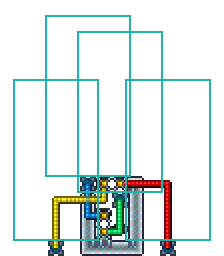
\includegraphics{images/254.png}
}
\end{center}
\caption{玩家试图左右移动时会触发玩家感应器并实化半砖将玩家推回;试图上平台时平台虚化,玩家掉落;试图下平台时下方半砖实化将玩家推回。}
\label{i253:254}
\end{figure}

\subsection{刷怪感应器}
刷怪感应器应用于刷怪场和Boss战场中,用来检测各种敌怪生成。大多数敌怪都可以直接触发压力板,所以一般情况下压力板就可以用来做刷怪感应器。穿墙怪不会触发压力板,只能使用特殊方法处理。

一个勉强及格的方案是在玩家周围放置压力板,穿墙怪攻击玩家时,玩家被击退,触发压力板,从而敌怪被检测到。这个方案的缺点是明显的,但是暂时也没有更好的方法。

\subsection{树感应器}
树感应器用于在树场中检测树的生成。当前景物块上方有树时,该前景物块无法被虚化。因此,可以使用制动器、飞镖机关和青绿压力垫板来检测树的生成。

\section{网线}

在设计大型电路时,有时会遇到需要在两地之间传递复杂信号的情况,例如在A地设置多个传感器,在B地进行处理并响应。一般来说每个信号都需要接一根线,这样一来当信号较复杂时,接线会占用非常大的空间。这是由于一根电线能传递的信号复杂度太低:一根电线只能选择激活或不激活两种状态,所以每根电线只能传递一个二进制位。

在了解了逻辑结算机制以后,我们可以使用一根电线传递多个二进制位。这个功能与现实生活中网线的功能类似,所以我把它称为网线。因为逻辑门是对逻辑帧敏感的,我们可以将多个二进制位在不同的逻辑帧通过一根电线发送出,并在接收端将这些信息解析。归根到底,我们需要做一个编码器和一个解码器。编码器用来把多根线上的简单信号翻译为一根线上的复杂信号,解码器用来将一根线上复杂信号翻译为多根线上的简单信号。

编码器和解码器的设计取决于信号特点,因此这里不给出固定的做法,仅给出一个简单例子作参考。我们在A地放置8根火把,使用开关可以改变它们的状态;在B地放置8根火把;A地和B地之间只能通过1根线连接。我们希望在设置完A地的火把之后,触发一个开关,就可以把A地的火把状态更新到B地,即利用一根线传递八个二进制位。

先考虑只有一个火把的情况,首先设置A火把,然后触发一个开关,使B火把和A火把同步。这个装置在数电上叫做D触发器。这个电路与置1/置0电路的区别不过是它的置1或置0是通过A火把的状态控制。我们只需要稍微修改一下置1/置0电路,就可以用一个逻辑门完成这个功能(\autoref{i237:238})。

\begin{figure}[!h]
\begin{center}
\subfloat{
\label{i237}

\includegraphics{images/237.png}
}
\qquad
\subfloat{
\label{i238}

\includegraphics{images/238.png}
}
\end{center}
\caption{左边的开关改变A火把的状态,右边的开关将A火把状态更新到B火把。}
\label{i237:238}
\end{figure}

那么对于8个火把的情况,我们只需要在8个逻辑帧中依次触发对应的D触发器,就可以把信号发送出去了(\autoref{i239:240})。

\begin{figure}[!h]
\begin{center}
\subfloat{
\label{i239}

\includegraphics{images/239.png}
}
\qquad
\subfloat{
\label{i240}

\includegraphics{images/240.png}
}
\end{center}
\caption{8个开关分别控制8个火把的状态,控制杆用来发送信号,黄线用来输出。第0个逻辑帧黄线激活,用来做启动信号,随后通过上方的逻辑延迟器,8个D锁存器依次在1\~{}8个逻辑帧激活。}
\label{i239:240}
\end{figure}

在B地,我们需要把各个逻辑帧的输入提取出来,然后分别输出给8个火把(\autoref{i241:242})。

\begin{figure}[!h]
\begin{center}
\subfloat{
\label{i241}

\includegraphics{images/241.png}
}
\qquad
\subfloat{
\label{i242}

\includegraphics{images/242.png}
}
\end{center}
\caption{接收到黄线(在第0个逻辑帧)的激活时开始工作。上方的逻辑延迟器依次在1\~{}8个逻辑帧将下方对应的有效逻辑灯点亮,对应逻辑帧时如果黄线激活,那么下方对应的火把被激活。第9个逻辑帧复位。}
\label{i241:242}
\end{figure}

以上的装置虽然使用了很多逻辑门,但是当AB两地距离较远时,使用这些逻辑门总比使用8根电线连接AB两地要好。

\section{传送阵}
传送阵,也就是传送机阵列,可以在多个传送机之间传送。根据功能不同,可以分为单向一传多、双向一传多、单向多传多、双向多传多、互传。根据操作方式,可以分为预设、一键和自动。预设指传送前需要通过多个操作设置传送目标;一键指激活一个开关就可以到对应的传送机;自动指不需玩家操作,在需要时自动传送。

阅读本节接下来内容之前请读者先熟悉\autoref{jiesuanshunxu}和\autoref{chuansongji}。

\subsection{利用传送机本身的大小}
传送机的大小是3*1,因此一个传送机上可以接出两根同色电线,所以简单地就可以做出双向一传八(\autoref{i243:244})。

\begin{figure}[!h]
\begin{center}
\subfloat{
\label{i243}

\includegraphics{images/243.png}
}
\qquad
\subfloat{
\label{i244}

\includegraphics{images/244.png}
}
\end{center}
\caption{传送机左边图格可以用四色电线接到四个不同传送机,右边图格可以用四色电线接到另外四个不同传送机。}
\label{i243:244}
\end{figure}

\subsection{利用传送区域大小}
一个传送机上的传送区域大小为3*3,因此多个传送机的传送区域可能重叠,当玩家站在重叠区域时可以被多个传送机传送,从而增加传送目标数(\autoref{i245:246})。

\begin{figure}[!h]
\begin{center}
\subfloat{
\label{i245}
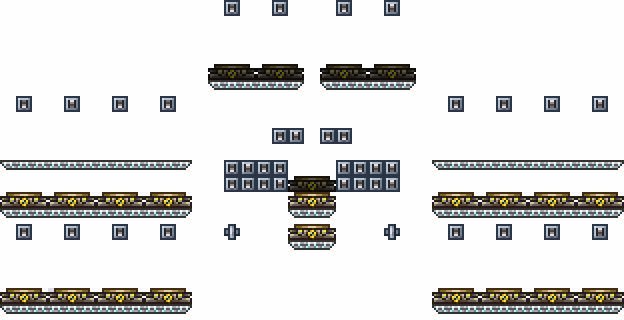
\includegraphics[width=0.95\textwidth]{images/245.png}
}
\qquad
\subfloat{
\label{i246}
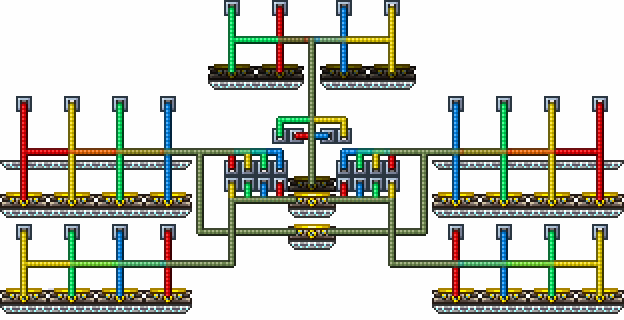
\includegraphics[width=0.95\textwidth]{images/246.png}
}
\end{center}
\caption{三个传送机的传送区域有三格重叠,当玩家站在重叠区域时可以传送到共20个其他传送机上。}
\label{i245:246}
\end{figure}

\subsection{用一根电线连接多个传送机}
当一根线连接了多个传送机图格时,只会在其中的两个图格间传送。至于是在哪两个图格之间传送,则取决于这根电线上的结算顺序,也就是取决于这根电线被激活的位置(具体规则详见\autoref{chuansongji})。利用这个特性,可以通过激活一根线上的不同位置来达到在指定传送机之间传送的目的(\autoref{i247:248})。

\begin{figure}[!h]
\begin{center}
\subfloat{
\label{i247}

\includegraphics[width=0.95\textwidth]{images/247.png}
}
\qquad
\subfloat{
\label{i248}
\includegraphics[width=0.95\textwidth]{images/248.png}
}
\end{center}
\caption{单向多传一。无论激活下面哪个传送机上的开关,第一个结算的传送机图格都是该开关正下方的图格,最后一个结算的传送机都是上方传送机的左图格或右图格。因此激活开关时会在上方传送机和下方对应传送机之间传送。}
\label{i247:248}
\end{figure}

\subsection{利用结算顺序}
在\autoref{jiesuanshunxu}中我们介绍了各种情况下电路的结算顺序。在这里我们将利用这些结算顺序来构造结构更复杂、功能更强大的传送阵。使用电线a连接传送机A和B,使用电线b连接传送机B和C,如果在电路结算中,a在b之前结算,那么站在传送机A上的玩家就会依次传送到B和C。在下一帧中,玩家会在C上出现,而B上只会出现传送的特效,玩家并不会触发B上的任何物理机制,例如受到熔岩伤害、触发加重压力板等。B在这里起到了中转的作用。利用多级中转可以实现非常复杂的传送功能。

首先来看一下如何利用结算顺序做中转(\autoref{})。

\begin{figure}[!h]
\begin{center}
\subfloat[]{
\label{i249:250}
\includegraphics[width=0.45\textwidth]{images/249.png}
\qquad
\includegraphics[width=0.45\textwidth]{images/250.png}
}
\qquad
\subfloat[]{
\label{i251:252}
\includegraphics[width=0.45\textwidth]{images/251.png}
\qquad
\includegraphics[width=0.45\textwidth]{images/252.png}
}
\end{center}
\caption{\protect\subref{i249:250}人物站在左边传送机上,右击左下开关,四个逻辑门从左到右依次激活,人物被依次传送到最右边;人物站在右边传送机上,右击右下开关或左上开关,四个逻辑门从右到左依次激活,人物被依次传送到最左边;\protect\subref{i251:252}原理与\protect\subref{i249:250}类似,只不过是利用了红蓝绿黄依次结算。}
\label{i249:252}
\end{figure}

利用传送链可以实现任意传送机互传(\autoref{})。

利用逻辑结算机制可以大大减少电路占地面积(\autoref{})。

\subsection{注记}
传送阵本身的功能是为了在多地之间快速旅行。如果违背了这个原则,那么传送阵的实用价值就要打折扣。例如预设置的传送阵(\autoref{})在操作上与简单的手控多级传送\autoref{}等价,但是建造成本却大大提高。在设计传送阵时不要迷恋表面上的传送数量,而是要结合用户体验和电路面积综合考量。对于更丰富的传送阵思路,请参考\url{https://www.bilibili.com/video/av24905110/}。

\section{显示器}
显示器从原理上分为分段显示器、密集矩阵显示器、稀疏矩阵显示器、像素盒显示器。

\subsection{分段显示器}
分段显示器,指根据显示需要,将显示界面分为若干部分分别控制的显示器。在显示器中有部分光源状态始终同步的情况下,将这些光源当作单个光源处理,即为一段。在十进制数显中我们将显示器分为了七段;在二进制数显中分为了两段;在\autoref{dianlujichu}的思考题中,将月相显示器的分段任务留给了读者。

分段之后就可以设计控制电路。\autoref{i42:43}和\autoref{i71}中展示了十进制数显的两种不同控制电路风格。前者逻辑门排列紧密,需要更多排换线器;后者逻辑门有间隔,需要换线器更少但是占用空间更大。由于显示部分本身体积就很小,使用占用空间大的控制电路容易导致接线难看(\autoref{i113:114})。

另外,\autoref{i42:43}和\autoref{i71}展示了十进制数显的两种不同分段方式。一个分段显示器可以有很多种分段方式,不同的分段方式对应不同的控制电路和接线。一个自然的问题是,是否可以设计出一个分段方式使得控制电路最简?答案是,没有一个固定的套路可以使控制电路最简。尽管如此,我们往往还是可以做出部分简化。下面以一个例子来介绍优化分段方式的方法。

我们希望修改十进制数显的分段来减少控制电路的大小。数显初始分段如\autoref{i34:35}所示。在这个分段下,数字与分段的对应关系如\autoref{sjzsxctjxdxsjz}。

\begin{table}[!h]
\centering
\begin{tabular}{c|ccccccc}
&a&b&c&d&e&f&g\\\hline
0&1&1&1&0&1&1&1\\
1&0&0&1&0&0&1&0\\
2&1&0&1&1&1&0&1\\
3&1&0&1&1&0&1&1\\
4&0&1&1&1&0&1&0\\
5&1&1&0&1&0&1&1\\
6&1&1&0&1&1&1&1\\
7&1&0&1&0&0&1&0\\
8&1&1&1&1&1&1&1\\
9&1&1&1&1&0&1&1
\end{tabular}
\caption{十进制数显传统接线的显示矩阵}\label{sjzsxctjxdxsjz}
\end{table}

上面的矩阵在$\mathbb{F}_2$\footnote{域$\mathbb{F}_2$包含0,1两个元素,可以将0看作偶数,1看作奇数。加法规则:0+0=1+1=0,0+1=1+0=1;乘法规则:0*0=0*1=1*0=0,1*1=1。}下的秩为7\footnote{后文中会介绍该矩阵的初等列变换操作并证明矩阵的列秩为7。},所以显示器至少要分成7段,没有办法减少段数。那么就没有可能减少控制电路中的换线器数量了吗?有的。在某些情况下,可以将同色的两段线连接到同一排换线器上并且使其不重叠(\autoref{})。用这种方法,7段线至多可以合并三对,这样就可以接在一行中。

我们对对应矩阵进行初等列变换,尝试将两列中的1分离。每列的列标是集合\{a,b,c,d,e,f,g\}的子集,列标为X的列的内容称为列X。初等列变换分为两种操作:
\begin{enumerate}
\item 交换列X和列Y,同时交换X和Y;
\item 将列X加到列Y上($\mathbb{F}_2$加法),同时将X改为X和Y的对称差\footnote{集合A与集合B的对称差定义为$A\triangle B=(A\cup B)-(A\cap B)$}。
\end{enumerate}

初等列变换过程如\autoref{bianhuanp1}和\autoref{bianhuanp2}。\autoref{bianhuanp1}使靠右的列的上部为0,经过这一步可以看出来矩阵的列秩为7;\autoref{bianhuanp2}使靠左的列的下部为0。经过变换后,第1列可以和第5列合并,第2列可以和第6列合并,第3列可以和第7列合并。合并后接线如\autoref{},注意由于合并的两列有重复段,在显示屏上不能使用同色电线,必须要使用额外的换线器。继续使用初等列变换可以减少换线器使用(\autoref{})。

\begin{figure}[p]
\centering
\subfloat[原矩阵]{
\label{bianhuan1}
\begin{tabular}{|c|ccccccc|}
&a&b&c&d&e&f&g\\\hline
0&1&1&1&0&1&1&1\\
1&0&0&1&0&0&1&0\\
2&1&0&1&1&1&0&1\\
3&1&0&1&1&0&1&1\\
4&0&1&1&1&0&1&0\\
5&1&1&0&1&0&1&1\\
6&1&1&0&1&1&1&1\\
7&1&0&1&0&0&1&0\\
8&1&1&1&1&1&1&1\\
9&1&1&1&1&0&1&1
\end{tabular}
}
\quad
\subfloat[将第1列加到第2,3,5,6,7列,交换第2,3列]{
\label{bianhuan2}
\begin{tabular}{|c|ccccccc|}
&abcefg&c&b&d&e&f&g\\\hline
0&1&0&0&0&0&0&0\\
1&0&1&0&0&0&1&0\\
2&1&0&1&1&0&1&0\\
3&1&0&1&1&1&0&0\\
4&0&1&1&1&0&1&0\\
5&1&1&0&1&1&0&0\\
6&1&1&0&1&0&0&0\\
7&1&0&1&0&1&0&1\\
8&1&0&0&1&0&0&0\\
9&1&0&0&1&1&0&0
\end{tabular}
}
\quad
\subfloat[将第2列加到第6列]{
\label{bianhuan3}
\begin{tabular}{|c|ccccccc|}
&abcefg&cf&b&d&e&f&g\\\hline
0&1&0&0&0&0&0&0\\
1&0&1&0&0&0&0&0\\
2&1&0&1&1&0&1&0\\
3&1&0&1&1&1&0&0\\
4&0&1&1&1&0&0&0\\
5&1&1&0&1&1&1&0\\
6&1&1&0&1&0&1&0\\
7&1&0&1&0&1&0&1\\
8&1&0&0&1&0&0&0\\
9&1&0&0&1&1&0&0
\end{tabular}
}
\quad
\subfloat[将第3列加到第4,6列,交换第4,5列]{
\label{bianhuan4}
\begin{tabular}{|c|ccccccc|}
&abcefg&cf&bdf&e&d&f&g\\\hline
0&1&0&0&0&0&0&0\\
1&0&1&0&0&0&0&0\\
2&1&0&1&0&0&0&0\\
3&1&0&1&1&0&1&0\\
4&0&1&1&0&0&1&0\\
5&1&1&0&1&1&1&0\\
6&1&1&0&0&1&1&0\\
7&1&0&1&1&1&1&1\\
8&1&0&0&0&1&0&0\\
9&1&0&0&1&1&0&0
\end{tabular}
}
\quad
\subfloat[将第4列加到第6列,交换第5,6列]{
\label{bianhuan5}
\begin{tabular}{|c|ccccccc|}
&abcefg&cf&bdf&ef&f&d&g\\\hline
0&1&0&0&0&0&0&0\\
1&0&1&0&0&0&0&0\\
2&1&0&1&0&0&0&0\\
3&1&0&1&1&0&0&0\\
4&0&1&1&0&1&0&0\\
5&1&1&0&1&0&1&0\\
6&1&1&0&0&1&1&0\\
7&1&0&1&1&0&1&1\\
8&1&0&0&0&0&1&0\\
9&1&0&0&1&1&1&0
\end{tabular}
}
\caption{}
\label{bianhuanp1}
\end{figure}

\begin{figure}[p]
\centering
\subfloat[将第6列加到第1,4,5列]{
\label{bianhuan6}
\begin{tabular}{|c|ccccccc|}
&abcefg&cf&bdf&ef&f&abcdfg&g\\\hline
0&1&0&0&0&0&0&0\\
1&0&1&0&0&0&0&0\\
2&1&0&1&0&0&0&0\\
3&1&0&1&1&0&0&0\\
4&0&1&1&0&1&0&0\\
5&0&1&0&0&1&1&0\\
6&0&1&0&1&0&1&0\\
7&0&0&1&0&1&1&1\\
8&0&0&0&1&1&1&0\\
9&0&0&0&0&0&1&0
\end{tabular}
}
\subfloat[将第5列加到第4列]{
\label{bianhuan7}
\begin{tabular}{|c|ccccccc|}
&abcefg&cf&bdf&ef&e&abcdfg&g\\\hline
0&1&0&0&0&0&0&0\\
1&0&1&0&0&0&0&0\\
2&1&0&1&0&0&0&0\\
3&1&0&1&1&0&0&0\\
4&0&1&1&1&1&0&0\\
5&0&1&0&1&1&1&0\\
6&0&1&0&1&0&1&0\\
7&0&0&1&1&1&1&1\\
8&0&0&0&0&1&1&0\\
9&0&0&0&0&0&1&0\\
\end{tabular}
}
\quad
\subfloat[将第7列加到第3,4,5,6列]{
\label{bianhuan8}
\begin{tabular}{|c|ccccccc|}
&abcefg&cf&bdf&ef&e&abcdfg&acf\\\hline
0&1&0&0&0&0&0&0\\
1&0&1&0&0&0&0&0\\
2&1&0&1&0&0&0&0\\
3&1&0&1&1&0&0&0\\
4&0&1&1&1&1&0&0\\
5&0&1&0&1&1&1&0\\
6&0&1&0&1&0&1&0\\
7&0&0&0&0&0&0&1\\
8&0&0&0&0&1&1&0\\
9&0&0&0&0&0&1&0
\end{tabular}
}
\subfloat[将第4列加到第2列]{
\label{bianhuan9}
\begin{tabular}{|c|ccccccc|}
&abcefg&cf&bdf&ce&e&abcdfg&acf\\\hline
0&1&0&0&0&0&0&0\\
1&0&1&0&0&0&0&0\\
2&1&0&1&0&0&0&0\\
3&1&1&1&1&0&0&0\\
4&0&0&1&1&1&0&0\\
5&0&0&0&1&1&1&0\\
6&0&0&0&1&0&1&0\\
7&0&0&0&0&0&0&1\\
8&0&0&0&0&1&1&0\\
9&0&0&0&0&0&1&0
\end{tabular}
}
\quad
\subfloat[将第2列加到第1列]{
\label{bianhuan10}
\begin{tabular}{|c|ccccccc|}
&abcefg&abeg&bdf&ce&e&abcdfg&acf\\\hline
0&1&0&0&0&0&0&0\\
1&1&1&0&0&0&0&0\\
2&1&0&1&0&0&0&0\\
3&0&1&1&1&0&0&0\\
4&0&0&1&1&1&0&0\\
5&0&0&0&1&1&1&0\\
6&0&0&0&1&0&1&0\\
7&0&0&0&0&0&0&1\\
8&0&0&0&0&1&1&0\\
9&0&0&0&0&0&1&0
\end{tabular}
}
\caption{}
\label{bianhuanp2}
\end{figure}

在上面的例子中,显示器在二进制输入为1010\~{}1111时会熄灭,也就是说显示器有十一种显示状态。如果我们不需要熄灭状态,减少一种状态,看看是否可以进一步减少换线器使用。

这里使用另一种技巧,我们先做一种预处理来减少矩阵中1的数量,这样有利于分离。定义矩阵列的反向操作:将该列列标的大小写互换,将该列01互换。标有大写的分段在接线时,其火把的01状态与正常情况相反。显然这个操作只有在初等列变换之前进行才有意义。

在初始的显示矩阵中,除了e列的1比0少,其他所有列的1都比0多,所以将其他所有列反向,可以减少矩阵中1的个数(\autoref{tab1})。对这个矩阵进行化简得到\autoref{},再作一些技巧上的处理(\autoref{}),就可以不使用换线器(\autoref{})。

\begin{table}[!h]
\centering
\begin{tabular}{c|ccccccc}
&a&b&c&d&e&f&g\\\hline
0&0&0&0&1&1&0&0\\
1&1&1&0&1&0&0&1\\
2&0&1&0&0&1&1&0\\
3&0&1&0&0&0&0&0\\
4&1&0&0&0&0&0&1\\
5&0&0&1&0&0&0&0\\
6&0&0&1&0&1&0&0\\
7&0&1&0&1&0&0&1\\
8&0&0&0&0&1&0&0\\
9&0&0&0&0&0&0&0
\end{tabular}
\caption{}\label{tab1}
\end{table}

此外,还有一些方法可以作为化简手段:
\begin{itemize}
\item 交换矩阵的行。在之前的操作中,控制0\~{}9的十个逻辑门是按照数字顺序排列的。在减少可读性的情况下,可以改变它们的顺序,而改变它们的顺序可能会使矩阵的列分离开。因为顺序改变了,所以由递次电路控制的数显不能用这种方法。
\item 将某一段用两根线控制。7段线合并3对可以放在一行内,8段线合并4对也可以放在一行内。这样的话可以将显示矩阵中有较多1的一段分成有较少1的两段,可能有利于分离。
\item 将多于两段合并。这种方法的局限性较强,因为它影响多层控制电路的接线。如果最终可以只化为1层,那么这种方法可用。
\end{itemize}

\subsection{密集矩阵显示器}
用单色光源可以实现至少有一边长度至多为4的密集显示器(\autoref{i256:257})。

\begin{figure}[!h]
\begin{center}
\subfloat{
\label{i256}
\includegraphics{images/256.png}
}
\qquad
\subfloat{
\label{i257}
\includegraphics{images/257.png}
}
\end{center}
\caption{第一行开关控制第一行火把,第二行开关控制第二行火把,第三行开关控制第三行火把,第四行开关控制第四行火把。}
\label{i256:257}
\end{figure}

\subsection{稀疏矩阵显示器}
稀疏矩阵显示器主要有两个参数:每个像素的光源面积与占用面积。稀疏矩阵显示器的大小不受限,一个典型的稀疏矩阵显示器如\autoref{i267:268}所示,当红线和蓝线在同一个逻辑帧输入时,火把响应,切换状态。显示器更新时,各行的红线逐次在各个逻辑帧激活,每列的蓝线在该逻辑帧选择性激活,用来控制该行的显示。这个例子中每个光源面积是4,占用面积是12,简称4占12,或4/12。目前使用这种显示器最杰出的作品是\url{https://www.bilibili.com/video/av22343683}。
\begin{figure}[!h]
\centering
\includegraphics{images/267.png}
\qquad
\includegraphics{images/268.png}
\caption{典型的矩阵显示器}
\label{i267:268}
\end{figure}

在这里我们看到控制每个像素的模块是一个占用3格的故障逻辑门。目前认为这是最小的控制单元\footnote{期待有人能开发出更小的显示器}。发光面积之间的间隔用来让控制的电线穿过。如果可以把火把摆在控制的电线上,那么就可以让显示器更紧凑(\autoref{i269:272})。
\begin{figure}[!h]
\begin{center}
\subfloat[6/9]{
\label{i269:270}
\includegraphics{images/269.png}
\qquad
\includegraphics{images/270.png}
}
\qquad
\subfloat[1/4]{
\label{i271:272}
\includegraphics{images/271.png}
\qquad
\includegraphics{images/272.png}
}
\end{center}
\caption{紧凑的矩阵显示器}
\label{i269:272}
\end{figure}

到这里你也许会有疑问,如果火把被摆在控制的电线上,不就会被控制的电线干扰吗?是的,是会被干扰,但是我们可以通过额外的激活来抵消这个干扰。具体说来,我们可以记录下每根控制电线激活的次数。如果一根控制电线激活了偶数次,那么它经过的火把是没有被干扰的。如果激活了奇数次,那么它经过的火把被取反,这时我们额外再激活一次这根线,就可以将火把恢复到没被干扰的状态。

接下来需要处理的一个问题是,额外激活的一次会不会干扰到某个像素?显然连接有效逻辑灯的电线不会,连接故障逻辑灯的电线可能会。事实上,如果我们先激活连接有效逻辑灯的电线,那么由于每根线都激活了偶数次,所有有效逻辑灯都会被关闭,此时再激活连接故障逻辑灯的电线不会干扰到任何一个像素。

此外,如果你足够细心,你会发现\autoref{i269:272}\subref{i271:272}中连接故障逻辑灯的电线也连接了有效逻辑灯,这不会出bug吗?在这种情况下,只要将有效逻辑灯的默认状态设为亮就行了。

还有一个非常巧妙的办法可以减少显示单元的面积,那就是使用小地图。半透明的小地图中每格2.5像素,在屏幕上是2像素和3像素交替排列。有很多使用小地图显示的例子:
\begin{itemize}
\item 【Terraria】做贪吃蛇—TheRedstoneCrafter \url{https://www.bilibili.com/video/av32265379}
\item 在Terraria中玩俄罗斯方块!? \url{https://www.bilibili.com/video/av38924330}
\end{itemize}

\subsection{像素盒显示器}

使用像素盒可以实现宽至多为24的密集矩阵显示器。因为其电路复杂,这里不给出电路图,仅给出原理。

首先来看如何更新屏幕状态。根据像素盒特性,显然每个像素盒都需要两个方向各一条线来控制,其中横向的线激活才会导致像素盒响应,仅纵向激活是不会响应的,这样一来屏幕的每行是独立的,可以逐行更新。

然后来看如何更新一行。当一行中的横向电线激活时,需要点亮的像素盒上的纵向电线必须被同一个电源激活,这意味着每个横向电线只能控制至多3个像素盒(\autoref{i258:259})。

\begin{figure}[!h]
\begin{center}
\subfloat{
\label{i258}
\includegraphics{images/258.png}
}
\qquad
\subfloat{
\label{i259}
\includegraphics{images/259.png}
}
\end{center}
\caption{八个开关分别将像素盒状态变为000,001,010,011,100,101,110,111。}
\label{i258:259}
\end{figure}

幸亏像素盒本身就有分线盒的作用,这样一来每行可以安排八个横向电线,更新这一行时从中间向两侧,每三个为一组更新(\autoref{i260})。

\begin{figure}[!h]
\centering
\includegraphics{images/260.png}
\caption{更新一行时,左边12个像素盒以3个为一组从右向左更新,右边12个像素盒以3个为一组从左向右更新。}
\label{i260}
\end{figure}

\section{自动化}

\section{思考题}
\begin{problemset}
\item 为什么在分段显示器的化简中对矩阵进行初等列变换时需要对列标做对称差?
\item 为什么两边长都大于4的非像素盒密集矩形随机显示器不存在?
\item 为什么像素盒显示器的宽度至多为24?
\end{problemset}